\documentclass[12pt,a4paper]{article}
\usepackage[utf8]{inputenc}
\usepackage[T1]{fontenc}
\usepackage[provide=*,french]{babel}
\usepackage{graphicx}
\usepackage{geometry}
\usepackage{hyperref}
\usepackage[all]{hypcap}
\usepackage{enumitem}
\usepackage{fancyvrb}

\geometry{margin=2.5cm}

\begin{document}

% Page de garde
\begin{titlepage}
    \begin{center}
        \vspace*{2cm}
        {\huge\bfseries Devoir 3\par}
        {INFO4305\par}
        \vspace{2cm}
        {\Large Alec Jones\par}
        {\large A00216262\par}
        \vfill
    \end{center}
\end{titlepage}

\tableofcontents
\newpage

% Introduction
\section{Introduction}
La cryptographie joue un rôle fondamental dans la sécurisation des communications numériques.
Dans ce document, nous explorons brièvement comment générer des clés,
chiffrer des messages et vérifier des signatures électroniques, afin de garantir l'intégrité et la confidentialité des échanges.

% Objectif
\section{Objectif du TP}
L'objectif de ce TP est de se familiariser avec la cryptographie à clé publique,
en particulier avec l'utilisation de GPG (GNU Privacy Guard) pour la gestion des clés et le chiffrement des messages.
Nous allons également aborder la création de certificats à l'aide d'OpenSSL et la signature de commits Git avec notre clé GPG.

% Corps du rapport
\newpage
\section{Déroulement du TP}
\subsection{Partie 1}
Premièrement on doit d'abord installer Gpg4win, j'ai installé le logiciel à
l'aide du cadre de paquets WinGet (voir la figure \ref{gpg4win}).

\begin{figure}[h]
    \centering
    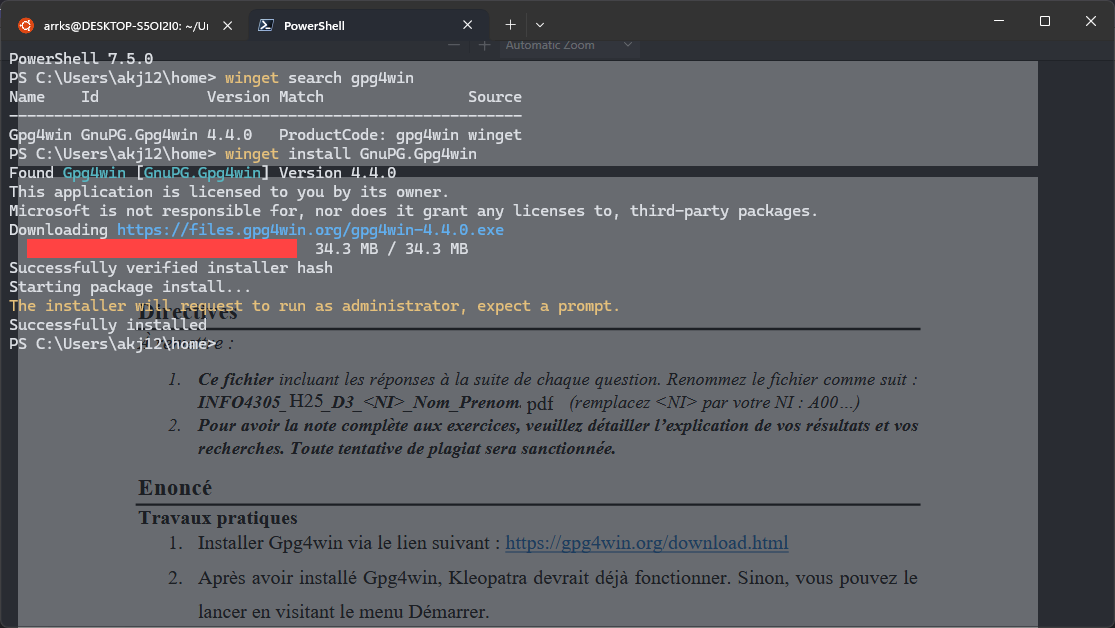
\includegraphics[width=0.8\textwidth]{../img/gpg4win.png}
    \caption{Installation de Gpg4win}
    \label{gpg4win}
\end{figure}

\subsection{Partie 2}
\subsubsection{Partie a}
Pour créer une paire de clés à l'aide de l'interface graphique, on doit ouvrir le logiciel
Kleopatra, ensuite on sélectionne l'option new key pair (voir la figure \ref{kleopatra}).

\begin{figure}[h]
    \centering
    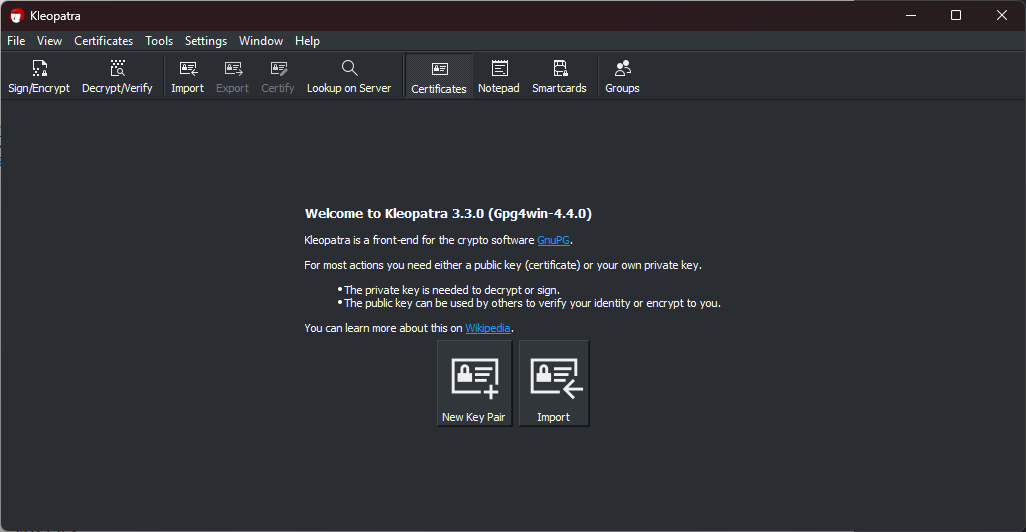
\includegraphics[width=0.8\textwidth]{../img/kleopatra.png}
    \caption{Menu initial Kleopatra}
    \label{kleopatra}
\end{figure}

Ensuite, on doit sélectionné options avancées et puis rsa2048.
On doit aussi remplir notre nom et notre courriel pour le certificat (voir \ref{newKey}).

\begin{figure}[ht]
    \centering
    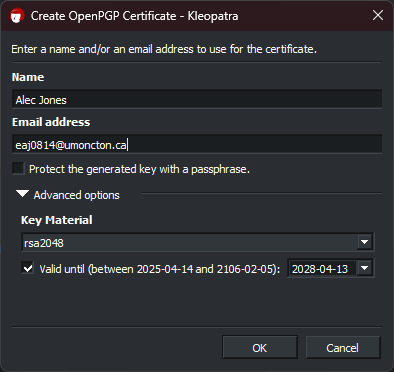
\includegraphics[width=0.8\textwidth]{../img/newKey.png}
    \caption{Création de clés dans Kleopatra}
    \label{newKey}
\end{figure}

\subsubsection{Partie b}
Pour créer une paire de clés en ligne de commande, vous pouvez utiliser la commande suivante dans un terminal :

\begin{verbatim}
gpg --full-generate-key
\end{verbatim}

Cette commande lance un assistant interactif vous permettant de choisir le type de clé, la longueur (par exemple, rsa2048 ou rsa4096)
et de renseigner les informations nécessaires (nom, adresse électronique, etc.). Une fois terminée, votre paire de clés sera générée et stockée dans votre trousseau GPG (voir figure \ref{newKey_cli}).

\begin{figure}[ht]
    \centering
    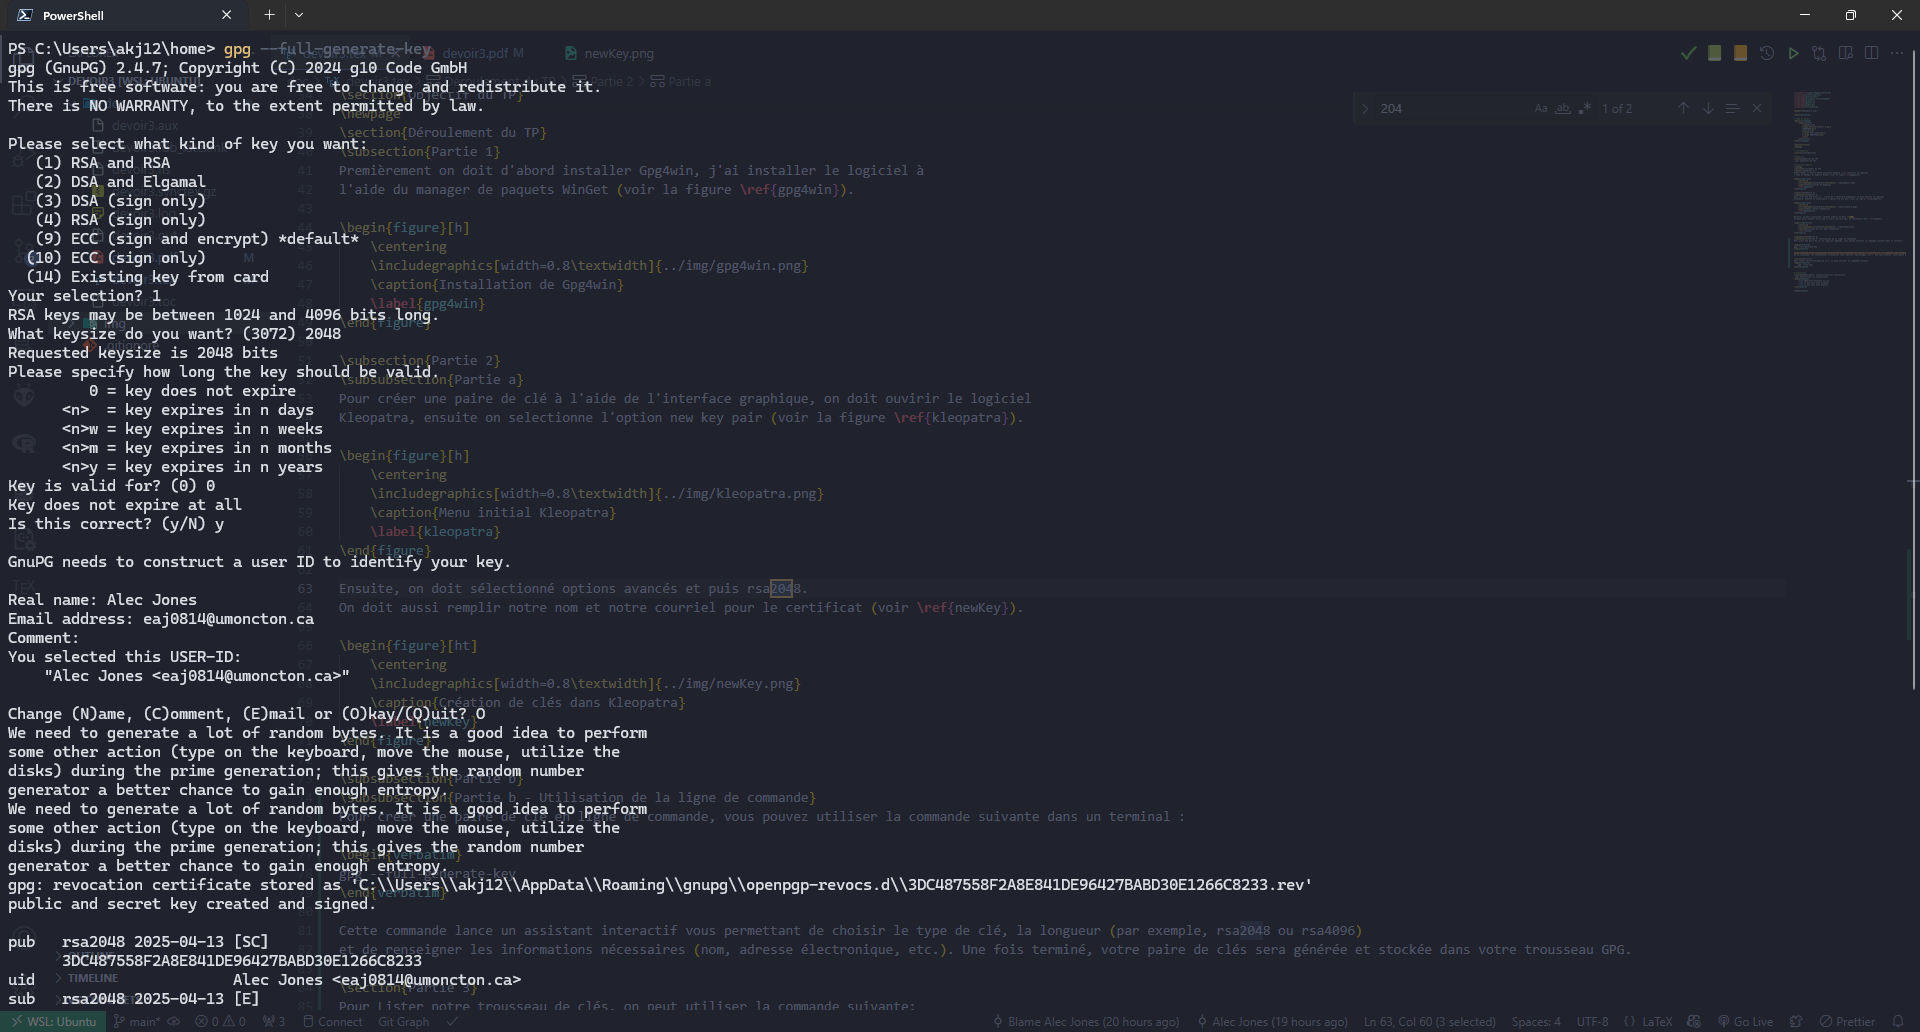
\includegraphics[width=0.8\textwidth]{../img/newKey_cli.png}
    \caption{Création de clés à l'aide de la ligne de commande}
    \label{newKey_cli}
\end{figure}

\subsection{Partie 3}
Pour lister notre trousseau de clés, on peut utiliser la commande suivante:
\begin{verbatim}
    gpg --list-keys
\end{verbatim}
En exécutant la commande, on aperçoit les deux clés créer précédemment (voir figure \ref{listKeys}).

\begin{figure}[ht]
    \centering
    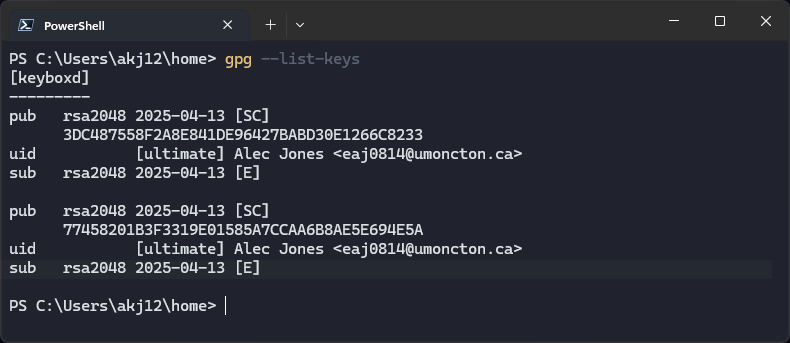
\includegraphics[width=0.8\textwidth]{../img/listKeys.png}
    \caption{Liste des clés}
    \label{listKeys}
\end{figure}

\subsection{Partie 4}
Pour exporter les clés publiques, on utilise la commande:
\begin{verbatim}
    gpg --armor --output maclé.asc --export UserID
\end{verbatim}
Puisqu'on spécifie le UserID, par exemple eaj0814@umoncton.ca,
qui a été utilisé dans les deux clés, on obtient la concaténation des deux dans un fichier.
On remarque alors que maclé.asc est effectivement la concaténation des deux clés publiques créée tout à l'heure.

\subsection{Partie 5}
Pour chiffrer un fichier, on utilise la commande suivante (voir figure \ref{chiffre} pour un exemple):
\begin{verbatim}
    gpg -er UserID document.txt
\end{verbatim}

\begin{figure}[ht]
    \centering
    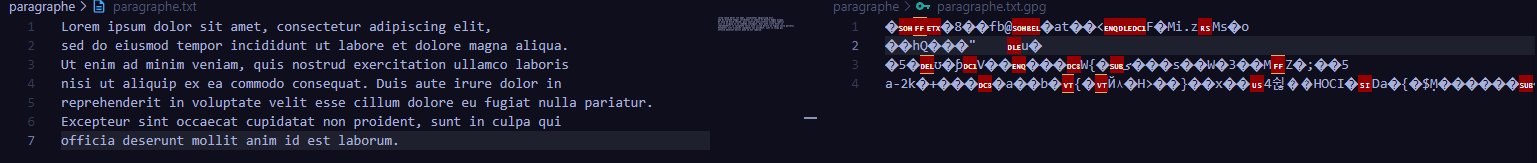
\includegraphics[width=0.8\textwidth]{../img/chiffre.png}
    \caption{texte clair à gauche, chiffré à droite}
    \label{chiffre}
\end{figure}

\subsection{Partie 6}
Si on voulait ensuite déchiffrer ce texte, on utiliserait la commande suivant :
\begin{verbatim}
    gpg --output doc --decrypt doc.gpg
\end{verbatim}

\subsection{Partie 7}
Pour signer un document et laisser le texte en clair, on utilise la commande suivante (voir la figure \ref{sign} pour exemple de résultat):
\begin{verbatim}
    gpg --clearsign document.txt
\end{verbatim}

\begin{figure}[ht]
    \centering
    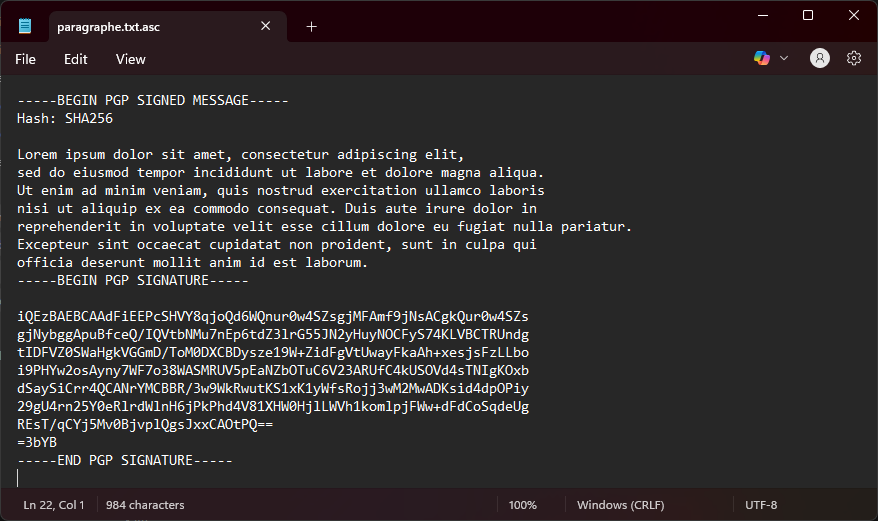
\includegraphics[width=0.8\textwidth]{../img/sign.png}
    \caption{Document signé}
    \label{sign}
\end{figure}

\subsection{Partie 8}
Pour vérifier la signature, on utilise la commande suivante (voir figure \ref{verif}):
\begin{verbatim}
    gpg --verify document.txt.asc
\end{verbatim}

\begin{figure}[ht]
    \centering
    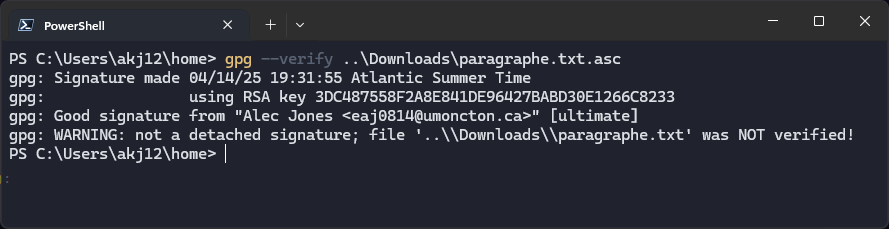
\includegraphics[width=0.8\textwidth]{../img/verif.png}
    \caption{Vérification de la signature}
    \label{verif}
\end{figure}

\subsection{Partie 9}
\subsubsection{Partie a}
L'utilité de la signature dans ce contexte est de garantir l'intégrité du document et d'assurer que le document n'a pas été modifié depuis sa signature.
En vérifiant la signature, on peut s'assurer que le document provient bien de la personne qui l'a signé et qu'il n'a pas été altéré.
(voir figure \ref{verif_modif} pour un exemple de document modifié).

\begin{figure}[ht]
    \centering
    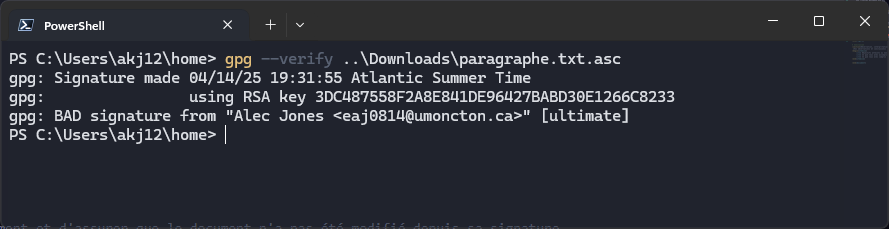
\includegraphics[width=0.8\textwidth]{../img/verif_modif.png}
    \caption{Vérification de la signature sur un document modifié, le premier mot a été enlevé}
    \label{verif_modif}
\end{figure}

\subsubsection{Partie b - Communication avec un camarade de classe}
\begin{enumerate}[label=\Roman*]
    \item Exporter votre clé publique. L'envoyer à un camarade de classe. J'ai réutilisé la commande suivante:
          \begin{verbatim}
        gpg --armor --output maclé.asc --export UserID
    \end{verbatim}
          J'ai ensuite envoyé le fichier maclé.asc à mon camarade de classe par courriel.

    \item Récupérer la clé publique de votre camarade et l'importer dans votre base de clés.
          Pour ce faire j'ai utilisé la commande suivante (voir figure \ref{import}):
          \begin{verbatim}
        gpg --import maclé.asc
    \end{verbatim}

          \begin{figure}[ht]
              \centering
              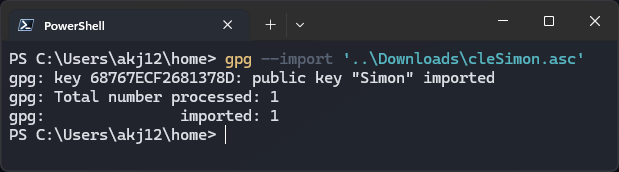
\includegraphics[width=0.8\textwidth]{../img/importCle.png}
              \caption{Importation de la clé publique de mon camarade}
              \label{import}
          \end{figure}


    \item Visualiser votre base de clés.
          Pour ce faire j'ai utilisé la commande suivante:
          \begin{verbatim}
        gpg --list-keys
    \end{verbatim}
          On remarque que la clé de mon camarade a bien été importée (voir figure \ref{listKeysSimon}).

          \begin{figure}[ht]
              \centering
              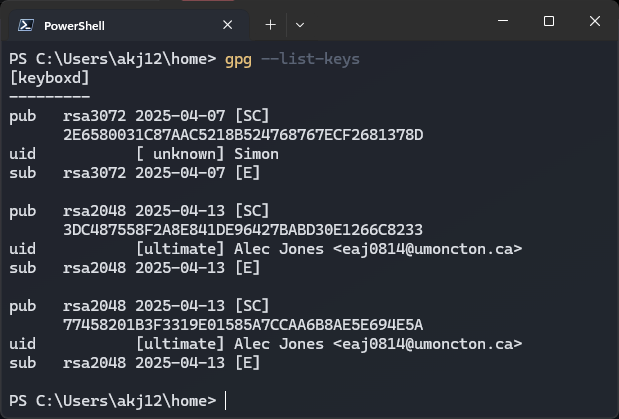
\includegraphics[width=0.8\textwidth]{../img/listKeysSimon.png}
              \caption{Liste des clés après importation de la clé publique de mon camarade}
              \label{listKeysSimon}
          \end{figure}

    \item Chiffrer un message à destination d'un camarade et lui envoyer.
          Pour ce faire j'ai utilisé la commande suivante:
          \begin{verbatim}
            gpg -er UserID paragraphe.txt
          \end{verbatim}
          J'ai ensuite envoyé le fichier paragraphe.txt.gpg à mon camarade de classe par Discord.

    \item Déchiffrer un message reçu d'un camarade.
          Pour ce faire j'ai utilisé la commande suivante (voir figure \ref{dechiffrer}):
          \begin{verbatim}
            gpg --decrypt doc.gpg
            \end{verbatim}

          \begin{figure}[ht]
              \centering
              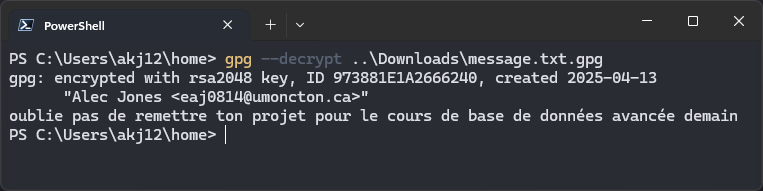
\includegraphics[width=0.8\textwidth]{../img/dechiffrer.png}
              \caption{Déchiffrement du message de mon camarade}
              \label{dechiffrer}
          \end{figure}

    \item Calculer la signature électronique d'un message et l'expédier à un camarade.
          Pour ce faire j'ai utilisé la commande suivante:
          \begin{verbatim}
                gpg --clearsign paragraphe.txt
            \end{verbatim}
          J'ai ensuite envoyé le fichier paragraphe.txt.asc à mon camarade de classe par Discord.

    \item Récupérer un message signé d'un camarade et vérifier sa provenance/intégrité.
          Après avoir reçu le message signé de mon camarade, j'ai utilisé la commande suivante pour vérifier la signature:
          \begin{verbatim}
                gpg --verify paragraphe.txt.asc
            \end{verbatim}
          On remarque que le message a bien été signé par mon camarade (voir figure \ref{verifSimon}).

          \begin{figure}[ht]
              \centering
              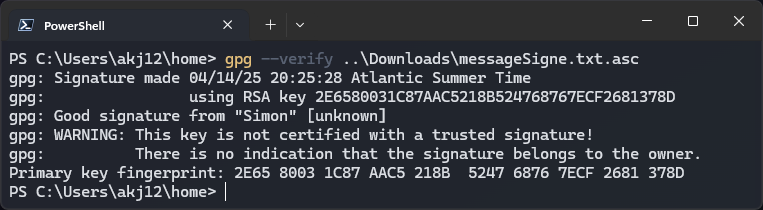
\includegraphics[width=0.8\textwidth]{../img/verifSimon.png}
              \caption{Vérification de la signature du message de mon camarade}
              \label{verifSimon}
          \end{figure}
\end{enumerate}

\subsection{Partie 10}
Pour créer un certificat à l'aide de openssl, on utilisera la commande suivante:
\begin{Verbatim}[fontsize=\footnotesize]
    openssl req -newkey rsa:2048 -keyout domain.key -out domain.csr
\end{Verbatim}

Décortiquons cette commande (voir figure \ref{opensslCert} pour la sortie):
\begin{itemize}
    \item \texttt{openssl req} : indique que nous voulons créer une demande de certificat.
    \item \texttt{-newkey rsa:2048} : crée une nouvelle clé RSA de 2048 bits.
    \item \texttt{-keyout domain.key} : Spécifie le fichier de sortie pour la clé privée.
    \item \texttt{-out domain.csr} : Spécifie le fichier de sortie pour la demande de signature de certificat (CSR).
    \item \texttt{-days 365} : Définit la durée de validité du certificat à 365 jours.
    \item \texttt{-sha256} : Utilise l'algorithme de hachage SHA-256 pour le certificat.
\end{itemize}

\begin{figure}[ht]
    \centering
    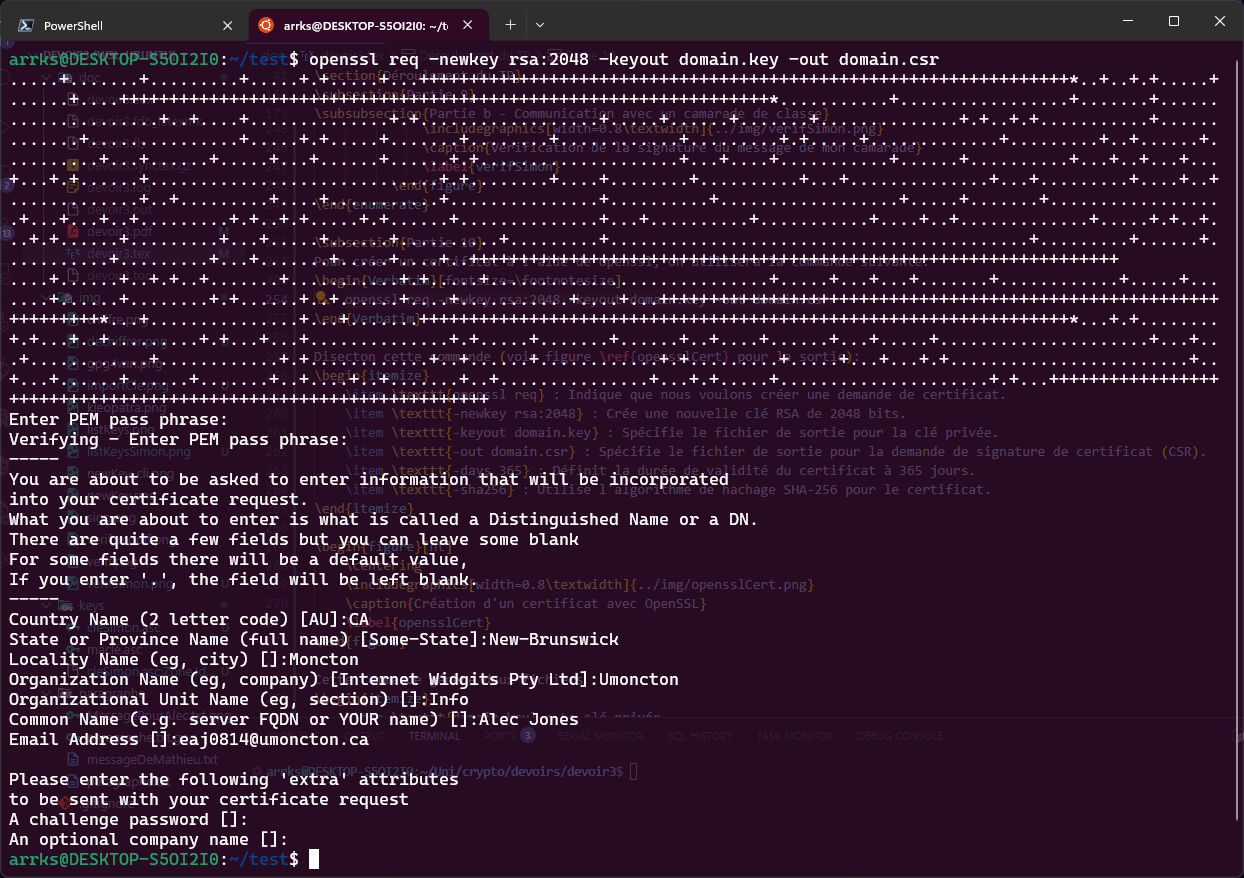
\includegraphics[width=0.8\textwidth]{../img/opensslCert.png}
    \caption{Création d'un certificat avec OpenSSL}
    \label{opensslCert}
\end{figure}

Cette commande génère deux fichiers :
\begin{itemize}
    \item \texttt{domain.key} : La clé privée.
    \item \texttt{domain.csr} : La demande de signature de certificat (CSR).
\end{itemize}

Normalement, ce serait à une autorité de certification (CA) de signer le certificat,
mais pour les besoins de ce TP, nous allons le signer nous-mêmes.

\subsection{Partie 11}
Pour signer le certificat avec la clé privée, on utilise la commande suivante:
\begin{Verbatim}[fontsize=\footnotesize]
    openssl x509 -signkey domain.key -in domain.csr -req -days 365 -out domain.crt
\end{Verbatim}

Décortiquons cette commande (voir figure \ref{opensslCertSign} pour la sortie):
\begin{itemize}
    \item \texttt{openssl x509} : Indique que nous voulons travailler avec des certificats X.509.
    \item \texttt{-signkey domain.key} : Spécifie la clé privée à utiliser pour signer le certificat.
    \item \texttt{-in domain.csr} : Spécifie le fichier d'entrée (CSR) à signer.
    \item \texttt{-req} : indique que nous travaillons avec une demande de signature de certificat.
    \item \texttt{-days 365} : Définit la durée de validité du certificat à 365 jours.
    \item \texttt{-out domain.crt} : Spécifie le fichier de sortie pour le certificat signé.
\end{itemize}

Cette commande génère un fichier \texttt{domain.crt} qui contient le certificat signé.
Ce certificat peut être utilisé pour établir des connexions sécurisées (SSL/TLS) sur un serveur web.

\begin{figure}[ht]
    \centering
    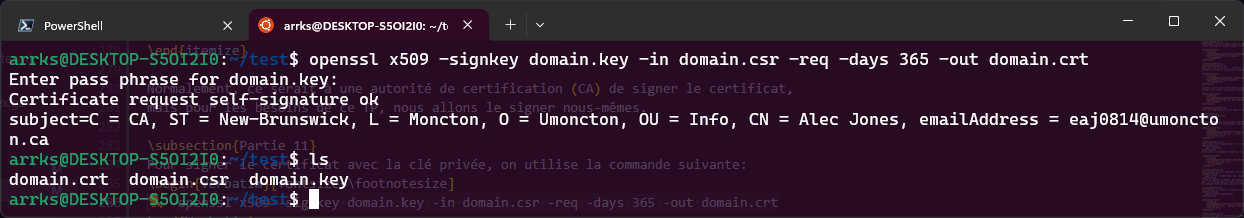
\includegraphics[width=0.8\textwidth]{../img/opensslCertSign.png}
    \caption{Signature d'un certificat avec OpenSSL}
    \label{opensslCertSign}
\end{figure}

\subsection{Partie 12}
Pour vérifier le certificat, on utilise la commande suivante:
\begin{Verbatim}[fontsize=\footnotesize]
    openssl x509 -texte -noout -in domain.crt
\end{Verbatim}

Décortiquons cette commande (voir figure \ref{opensslCertVerif} pour la sortie):
\begin{itemize}
    \item \texttt{openssl x509} : indique que nous voulons travailler avec des certificats X.509.
    \item \texttt{-texte} : Affiche les informations du certificat de manière lisible.
    \item \texttt{-noout} : N'affiche pas le contenu brut du certificat.
    \item \texttt{-in domain.crt} : spécifie le fichier d'entrée (certificat) à vérifier.
\end{itemize}

Cette commande affiche les informations du certificat,
y compris le nom du sujet, la clé publique, la période de validité et d'autres détails.

\begin{figure}[ht]
    \centering
    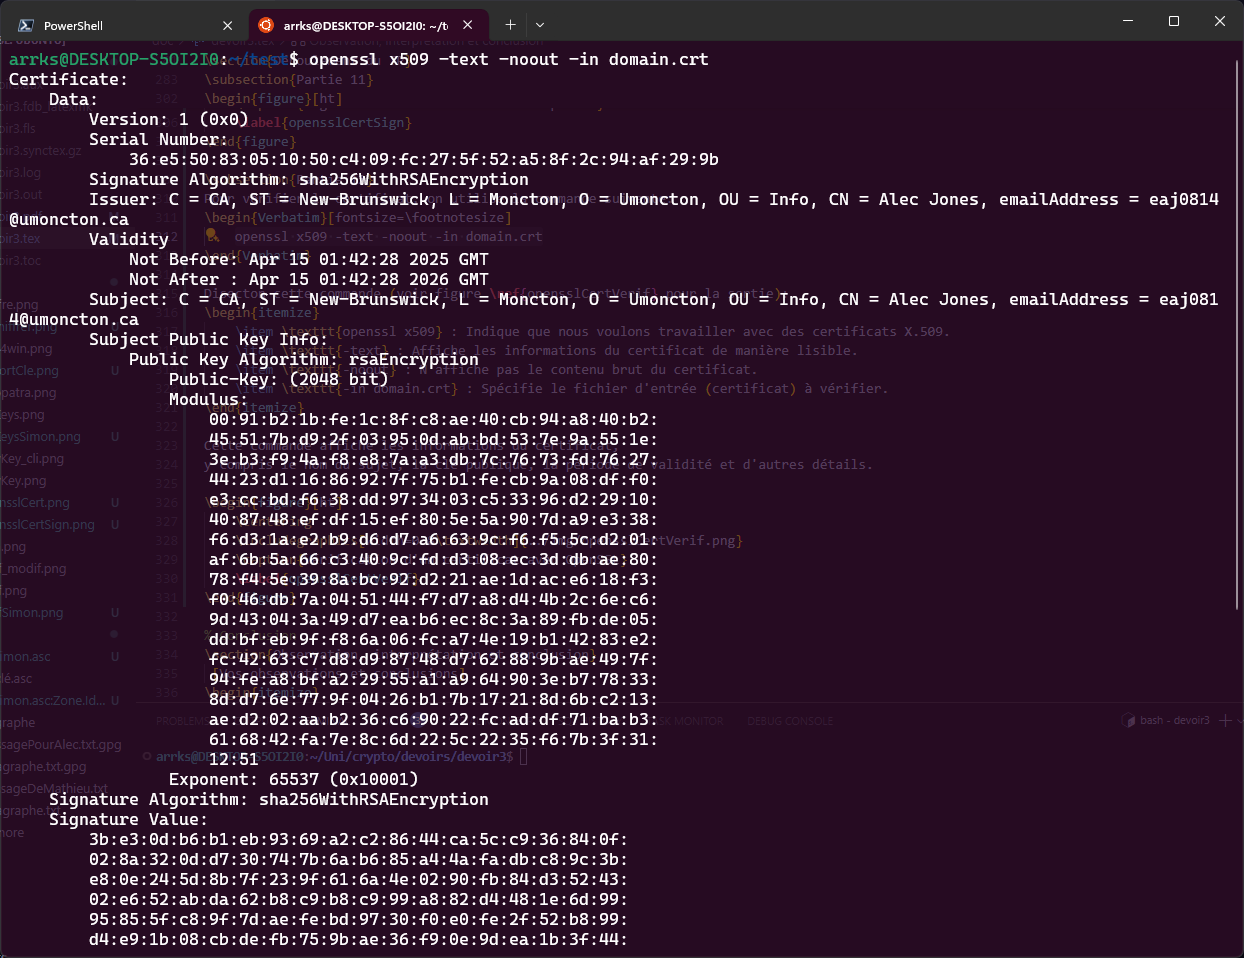
\includegraphics[width=0.8\textwidth]{../img/opensslCertVerif.png}
    \caption{Vérification d'un certificat avec OpenSSL}
    \label{opensslCertVerif}
\end{figure}

\subsection{Partie 13}
Git est un système de contrôle de version distribué qui permet de suivre
les modifications apportées à des fichiers et de collaborer avec d'autres personnes.
On est aussi capable de signer nos commits avec notre clé privée GPG.
Pour ce faire, on doit d'abord configurer git pour utiliser notre clé GPG.

Premièrement, on doit lsiter nos clés GPG pour trouver l'ID de notre clé publique.
Ensuite, on doit configurer git pour utiliser cette clé avec les commandes suivantes:
\begin{verbatim}
    git config --global user.signingkey <ID de la clé>
    git config --global commit.gpgsign true
\end{verbatim}

Ensuite, on peut signer nos commits avec la commande suivante:
\begin{verbatim}
    git commit -S -m "Message de commit"
\end{verbatim}

Le -S indique à git de signer le commit avec notre clé GPG.
On peut vérifier la signature du commit avec la commande suivante:
\begin{verbatim}
    git log --show-signature
\end{verbatim}

On devra aussi s'assurer que notre clé publique est disponible sur GitHub pour que les autres
pouvant vérifier la signature de nos commits.
Pour ajouter notre clé publique à GitHub, on doit se rendre dans les paramètres de notre compte,
aller dans la section "SSH and GPG keys" et cliquer sur "New GPG key" (voir figure \ref{gitGPG}).

\begin{figure}
    \centering
    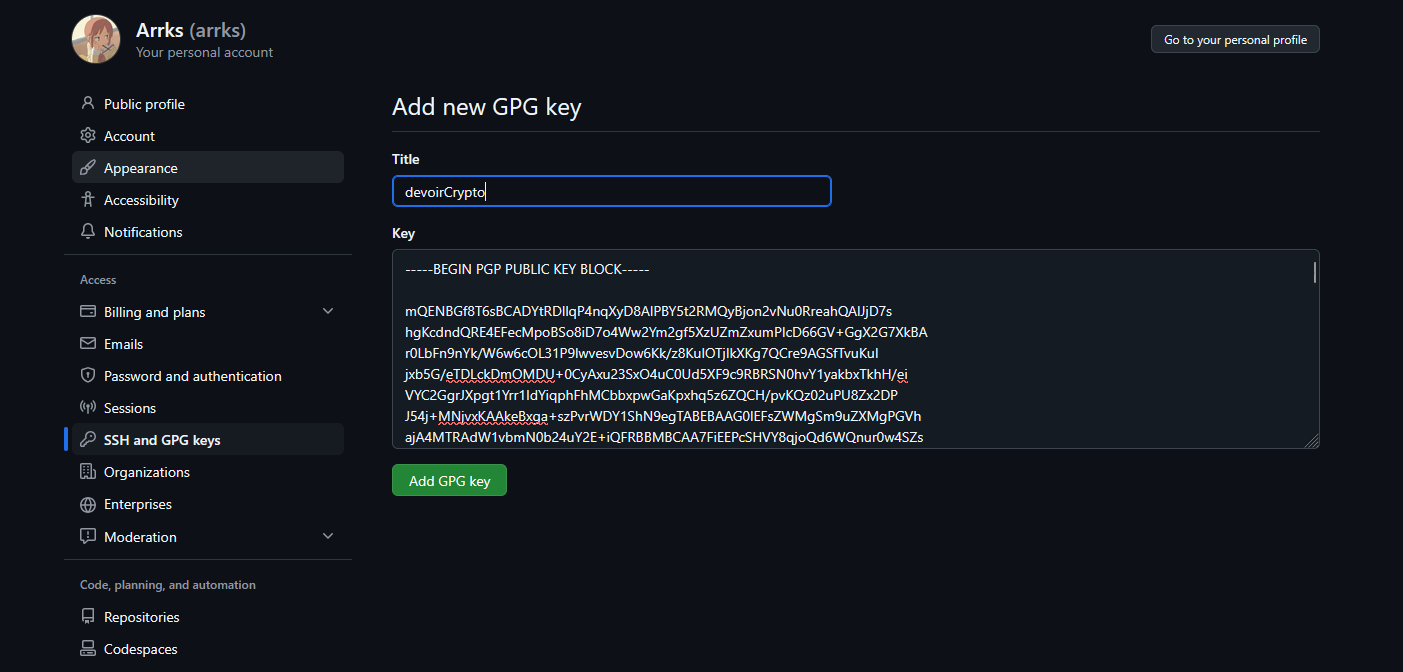
\includegraphics[width=0.8\textwidth]{../img/gitGPG.png}
    \caption{Ajout de la clé publique à GitHub}
    \label{gitGPG}
\end{figure}

Après avoir effectué un push à GitHub, on peut vérifier que notre commit est bien signé
en se rendant sur la page des commits sur GitHub (voir figure \ref{gitGPGVerif}).
\begin{figure}
    \centering
    
\includegraphics[width=0.8\textwidth]{../img/githubVerified.png}
    \caption{Vérification de la signature du commit sur GitHub}
    \label{gitGPGVerif}
\end{figure}

% Conclusion
\section{Observation, interprétation et conclusion}
Dans ce TP, nous avons exploré les concepts fondamentaux de la cryptographie à clé publique,
y compris la génération de clés, le chiffrement et le déchiffrement de messages,
la signature électronique et la vérification de signatures.
Nous avons également appris à utiliser GPG pour gérer nos clés et signer nos commits Git,
ainsi qu'à créer et signer des certificats avec OpenSSL.
Ces compétences sont essentielles pour garantir la sécurité et l'intégrité des communications numériques,
en particulier dans le contexte de la collaboration en ligne et du développement de logiciels.

\section{Sources}
\begin{itemize}
    \item GNU Privacy Guard (GPG): \url{https://gnupg.org/}
    \item OpenSSL: \url{https://www.openssl.org/}
    \item Documentation Git: \url{https://git-scm.com/doc}
    \item Aide poru certificats: \url{https://www.baeldung.com/openssl-self-signed-cert}
\end{itemize}

\end{document}
